\documentclass{article}
\usepackage{fullpage,amsmath,amsthm,graphicx,enumitem}
\usepackage{multicol}
\usepackage{booktabs}
\usepackage{blkarray}

\usepackage{tikz}

\theoremstyle{definition}
\newtheorem{thm}{Theorem}
\newtheorem{question}[thm]{Question}
\newenvironment{solution}{\noindent\textit{Solution:}}{}

\title{ASEN 5264 Decision Making under Uncertainty\\
       Quiz 3: Games and Conditional Independence in Bayesian Networks}

\date{\small Show all work and justify and box answers.\\
You may consult any source, but you may NOT communicate with any person except the instructor. If you do not understand how to do a problem, MOVE ON and come back to finish later so that you attempt all problems.
}

\begin{document}
\maketitle

\begin{question} (40 pts)
    \begin{enumerate}[label=\alph*)]
        \item Find the pure Nash equilibria in the following game:
            \begin{center}
                \begin{tabular}{cc}
                & Player 2\\
                    Player 1 & 
            \begin{tabular}{c|c|c|}
            & a & b \\ \hline
            a & 5,4 & 2,3 \\ \hline
            b & 4,1 & 3,2 \\ \hline
            \end{tabular}
                \end{tabular}
            \end{center}
        \item Does the game above have a dominant strategy equilibrium? Justify your answer.
        \item Choose values for $x$ and $y$ in the simple game below so that there are no pure Nash equilibria:
            \begin{center}
                \begin{tabular}{cc}
                & Player 2\\
                    Player 1 & 
            \begin{tabular}{c|c|c|}
            & a & b \\ \hline
            a & $2, x$ & $3, 1$ \\ \hline
            b & $3, 1$ & $y, 2$\\ \hline
            \end{tabular}
                \end{tabular}
            \end{center}
        \item Does the game above (that you created) have a Nash equilibrium? How do you know?
    \end{enumerate}
\end{question}

\begin{question} (30 pts)
    Consider the following Bayesian network structure:

    \begin{center}
    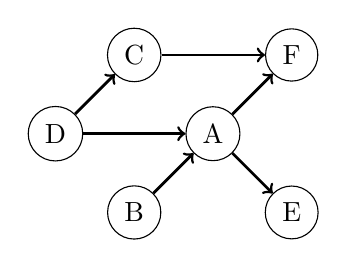
\begin{tikzpicture}
        \node[shape=circle,draw=black] (D) at (0,0) {D};
        \node[shape=circle,draw=black] (A) at (2,0) {A};
        \node[shape=circle,draw=black] (C) at (1,1) {C};
        \node[shape=circle,draw=black] (F) at (3,1) {F};
        \node[shape=circle,draw=black] (E) at (3,-1) {E};
        \node[shape=circle,draw=black] (B) at (1,-1) {B};
        \path [->,line width=1pt] (D) edge node[left]{}(A);
        \path [->,line width=1pt] (D) edge node[left]{}(C);
        \path [->,line width=1pt] (B) edge node[left]{}(A);
        \path [->,line width=1pt] (A) edge node[left]{}(E);
        \path [->,line width=1pt] (A) edge node[left]{}(F);
        \path [->,line width=1pt] (C) edge node[left]{}(F);
    \end{tikzpicture}
    \end{center}

    \begin{enumerate}[label=\alph*)]
        \item Is it possible to conclude from the structure that $B \perp F \mid D$? Justify your answer.
        \item Is it possible to conclude from the structure that $B \perp F \mid A$? Justify your answer.
        \item Is it possible to conclude from the structure that $B \perp E \mid A$? Justify your answer.
    \end{enumerate}
\end{question}

\clearpage

\begin{question} (20 pts)
    Consider a Markov game with two players, $\mathcal{I}=\{1,2\}$ and three states, $\mathcal{S}=\{1,2,3\}$. Each player can play $0$ or $1$, i.e. $\mathcal{A}^1 = \mathcal{A}^2 = \{0,1\}$. The game is zero sum, so $R^1(s, a) = -R^2(s, a)$. Player 2 gets a point if $s=2$, otherwise, there is no reward, i.e.
    \begin{equation}
        R^2(s, a) = \begin{cases}
            1 &\text{ if } s = 2 \\
            0 &\text{ otherwise.}
        \end{cases}
    \end{equation}
    The state deterministically transitions according to $s' = s + a^1 + a^2$ stopping at state $3$, that is
    \begin{equation}
        T(s' \mid s, a^1, a^2) = \begin{cases}
            1 &\text{ if } s' = \min(s + a^1 + a^2, 3) \\
            0 &\text{ otherwise,}
        \end{cases}
    \end{equation}
    and there is no discounting, $\gamma = 1.0$.
    Now suppose that Player 1 adopts a strategy $\pi^1$ that always plays $1$ in states $2$ and $3$, but plays 0 with $80\%$ probability in state 1.
    \begin{equation}
        \pi^1(a^1 \mid s) = \begin{cases}
            1 &\text{ if } s \in \{2, 3\} \text{ and } a^1 = 1 \\
            0.8 & \text{ if } s = 1 \text{ and } a^1 = 0 \\
            0.2 & \text{ if } s = 1 \text{ and } a^1 = 1 \\
            0.0 & \text{ otherwise.}
        \end{cases}
    \end{equation}
    \begin{enumerate}[label=\alph*)]
        \item If the current state is 1 and Player 1 plays according to $\pi^1$ and Player $2$ plays $a^2=1$, what is the probability that the next state will be 2?
        \item Describe in two steps how to find player 2's best response to $\pi^1$.
        \item Find player 2's best response to $\pi^1$ at state 1. (Hint: since neither player receives reward in state 3 and it is impossible to move out, state 3 can be considered terminal.)
    \end{enumerate}
\end{question}

\begin{question} (5 pts)
    Consider a two player Markov game and policy $\pi^1$ for player 1. Suppose that player 2 computes a best response to $\pi^1$ and call that policy $\pi^2$. Now, let $\pi^{1*}$ be a best response to $\pi^2$. Can we conclude that the joint policy $(\pi^{1*}, \pi^{2})$ is a Nash equilibrium? Why or why not?
\end{question}

\begin{question} (5 pts)
    Consider the extensive-form game tree discussed in class. Suppose that player 2 is not allowed to see \emph{any} cards, that is, he or she is dealt a card, but must keep it face down without looking. How would the extensive form game tree for this new game be different from the original game displayed below? You can draw or briefly describe your answer in words.

    \vspace{1em}
    \includegraphics[height=7cm]{efg.png}
\end{question}

% \begin{question} (30 pts)
%     Answer the following questions about simple games:
%     \begin{enumerate}[label=\alph*)]
%         \item Does the following game have a Nash equilibrium? Justify your answer.
%             \begin{center}
%                 \begin{tabular}{cc}
%                 & Player 2\\
%                     Player 1 & 
%             \begin{tabular}{c|c|c|}
%             & a & b \\ \hline
%             a & 1,2 & 2,1 \\ \hline
%             b & 2,1 & 1,2 \\ \hline
%             \end{tabular}
%                 \end{tabular}
%             \end{center}
%         \item Consider the following incomplete game matrix:
%             \begin{center}
%                 \begin{tabular}{cc}
%                 & Player 2\\
%                     Player 1 & 
%             \begin{tabular}{c|c|c|}
%             & a & b \\ \hline
%             a & 10,10 & 3,5 \\ \hline
%             b & 5,3 & $x$,$y$ \\ \hline
%             \end{tabular}
%                 \end{tabular}
%             \end{center}
%             Choose $x$ and $y$ so that the game has two pure Nash equilibria.
%         \item In the incomplete game matrix above, choose $x$ and $y$ so that the game has a single dominant strategy equilibrium.
%     \end{enumerate}
% \end{question}

% \begin{question} (30 pts)
%     Consider a turn taking game where Player 1 (the maximizing player) chooses a number between 1 and 3 (i.e. 1, 2, or 3) then, after seeing Player 1's number, Player 2 also chooses a number between 1 and 3. If \emph{both} the sum of the two numbers \emph{and} the product of the two numbers are even, Player 2 wins, otherwise, Player 1 wins.
%     \begin{enumerate}[label=\alph*)]
%         \item Draw a minimax tree depicting this game labeled with payoffs.
%         \item Use minimax backup to calculate the values at each node and indicate them on the tree.
%         \item Which player has the advantage?
%         \item What number should Player 1 choose?
%     \end{enumerate}
% \end{question}

\end{document}
